%General formatting
\documentclass[oneside]{book}
\usepackage{amssymb,latexsym,color,amsthm}
\usepackage[margin=1.5in]{geometry}

%allows for comment blocks and verbatim sections
\usepackage{verbatim}
%For links
\usepackage{hyperref}
%For inserting images
\usepackage{graphicx}
%preserves tabs in verbatim sections. Good for including source code in documents.
\usepackage{moreverb}

%For examples
\definecolor{Dark}{gray}{.20}
\definecolor{Light}{gray}{.80}
\newcommand{\commandline}[1]{\begin{center} \colorbox{Dark}{\textcolor{white}{#1}} \end{center}}
\newcommand{\exampleout}[1]{\begin{center} \colorbox{Light}{\textcolor{black}{#1}} \end{center}}

%For exercises                          (Could be made prettier)
\newtheorem{ex}{Exercise}[chapter]

% code block formatting
\usepackage{listings,color}
\definecolor{verbgray}{gray}{0.9}
\definecolor{shadecolor}{rgb}{.9, .9, .9}
\lstnewenvironment{code}{
    \lstset{backgroundcolor=\color{verbgray}, 
    frame=single,
    framerule=0pt,
    basicstyle=\ttfamily,
    columns=fullflexible}}{}


\begin{document}
%Title Page
\title{An Introduction to the UNIX Command Line}
\author{Brandon Tarquinio and Sarah Gunderson}

\maketitle
\tableofcontents
\newpage

                                                        %Workshop 2
\chapter{Advanced Shell Use}
Now that we have built some familiarity with the command line and know the basics of files and directories, we are ready to build our repertoire of commands and learn the more advanced features of the shell and UNIX. Therefore we will assume familiarity with everything covered in the last chapter.

\section{Permissions and chmod}
In the previous chapter we learned how to list the files in a directory and how to read, copy, move, remove, and create files. All of these files we were manipulating have a set of permissions associated with them. These permissions allow a user to restrict what people are allowed to do with their files, including restricting what the user themselves can do with the file. 
\subsection{How to check permissions}
If every file has permissions then how can we see them? The program \textbf{ls} comes to the rescue again with the the \textbf{-l} argument which is short for \textbf{l}ong format. If we run:
\commandline{ls -l}
We get a list of entries of the following form:
\exampleout{permissions hardLinkCount owner'sUsername groupname size lastModifiedDate fileName}
Let's examine what this all means with an example:
\commandline{ls -l}
This command produces the following output:
\exampleout{total 0}
\exampleout{-rw-r--r--  1 tarquinio  staff  0 Feb 12 15:47 file1}
Therefore $ls -l$ shows us a lot of information about our files that is suppressed when we run $ls$. Let's break down what all this new information means:
\begin{itemize}
    \item{1:} This states that there is only one hardlink to this file. We will learn more about hardlinks later.
    \item{tarquinio:} This is the username of the owner of this file.
    \item{staff:} The associated group of the owner of this file is ''staff".
    \item{0:} This file is 0 bytes long.
    \item{Feb 12 15:47:} This file was last modified on this date (This might be useful if there is a grade dispute with your teacher in deciding if you did finish your project before it was due).
    \item{file1:} The name of the file.
    \item{-rw-r--r--:} This is the permission flags which can we will break down now.
\end{itemize}
The permission flags will always have this form:
\begin{enumerate}
    \item The left most flag designates the type of the file. Here are some examples:
        \begin{itemize}
            \item{`` - ":} states the file is a text file.
            \item{`` d ":} states the file is a \textbf{d}irectory.
            \item{`` l ":} the file is a symbolic \textbf{l}ink.
            \item{`` c ":} \textbf{c}haracter device (We will not cover this or the few other file types in the workshop).
        \end{itemize}
    \item The file type bit is proceeded by three groups of three bits with the groups being in the following order: owners permissions, group's permissions, and other's permission (other is any user who is not the owner or in the group associated with the file). The three bits are broken down from left to right as follows:
        \begin{itemize}
            \item{`` w/- ":} w is for write permission, - is for no write permission.
            \item{`` r/- ":} r is read permission, - is no read permission.
            \item{`` x/- ":} x is execute permission, - is no execute permission.
        \end{itemize}
\end{enumerate}
We can now interpret what -rw-r--r-- for $file1$ stands for. $file1$ is a regular text file that has \textbf{r}ead and \textbf{w}rite permissions for the owner, only \textbf{r}ead permissions for users in it's associated group, and only \textbf{r}ead permission for any other user.

\begin{ex}
    Suppose we make a new file $myFirstShellScript.sh$ which is your first shell script. You would like to be able to do whatever you want with it and are quite excited so you would like all the other students to be able to read and run it as well. But you don't want anyone else to change it and want non-students to not be allowed to do anything with it. What should the permission flag for this new file be? 
\end{ex}

\begin{ex}
    In this exercise we explore ``ls -l" more and revisit \textbf{touch}.
    \begin{itemize}
            \item Examine your files using the long format. Thus,
                \commandline{ls -l}
            \item Pick a file, say file1, and run the following:
                \commandline{touch file1}
            \item Examine the file again using:
                \commandline{ls -l}
            \item Has anything changed? How could this be useful?
    \end{itemize}
\end{ex}

\begin{ex}
    We mentioned that there are other files than just regular files and directories. See for yourself by running the following command:
        \commandline{ls -l /dev}
    How can we tell that these files, for the most part, are neither a regular file nor a directory? What did we find? Also pay attention to their group owners since some of these will new to you.
\end{ex}

\subsection{What are groups?}
We now know that every file has an associated group and has a set of permission bits for what user's in that group can do with the file. But what are groups?

We can see all groups a certain user is in with the following command:
\commandline{groups username}
So on the lab computers you can type:
\commandline{groups tarquib}
And get:
\exampleout{tarquib : grp.csci.Students}
Which shows that my account is part of the computer science student group. On some systems you will be in more than just one group such as admin, ect. If you enter:
\commandline{groups}
It will default to showing you what groups you are associated with. Thus if you set read permissions on a file for group then all other students will be able to read that file.

\subsection{Changing permissions}
Now that we understand how to find and interpret permissions on files let's learn how to change them. The command \textbf{chmod} allows us to \textbf{ch}ange the \textbf{mod}e of a file which is UNIX jargon for change the files permission.
The command has the following generic form:
\commandline{chmod permissions file1 file2 ...}
Where permission has the form $d_1d_2d_3$ such that each $d$ is between zero and seven. As you might have guessed $d_1$ is for user, $d_2$ is for group, and $d_3$ is for other. We compute the numbers as follows: \\
\begin{center}
\begin{tabular}{|c|c|}
    \hline
    1 & Execute  \\ 
    2 & Write   \\ 
    4 & Read \\ \hline
\end{tabular}
\end{center}

So to have read, write, and execute for the owner but nothing for the group and only read and write for others we would have $d_1 = 1 + 2 + 4 = 7$, $d_2 = 0$, and $d_3 = 2 + 4 = 6$. The corresponding command to change $theFile$ to have these permissions is:
\commandline{chmod 706 theFile}

\begin{ex}
    We talked about the permissions for $myFirstShellScript.sh$ before. Let's now make our first shell script and set the permissions using $chmod$. Our shell script will print ``Hello World!".
    \begin{itemize}
        \item Make the file, using vim or nano, whose content should be only this line:
            \exampleout{echo "Hello World!"}
        \item Save and exit the file.
        \item Check the default permissions.
        \item Use chmod to change the permissions to the one's you came up with in the previous exercise; they should have been ``-rwxr-x---".
        \item Run the script by typing the following:
            \commandline{./myFirstShellScript.sh}
    \end{itemize}
\end{ex}

\begin{ex}
    Shell scripts are important so to give a better idea of them we will make one more that determines how to greet you. 
    \begin{itemize}
        \item Make the file ``greeting.sh", using vim or nano, with the following content:
\begin{verbatimtab}
#!/bin/bash
echo -n "Is it before noon (y/n)? "
read beforeNoon

if [ "$beforeNoon" == "y" ]; then
    echo "Good Morning!"
else
    echo "Good Afternoon!"
fi
\end{verbatimtab}
        \item Add execute permissions by running the following:
            \commandline{chmod +x greeting.sh}
        \item Run it by entering:
            \commandline{./greeting.sh}
    \end{itemize}
\end{ex}


\section{Grep!}
    Grep is used to find occurrences of anything that matches a given regular expression in a file. 
\subsection{Regular expressions}
    There is an entire formal language known as Regular expressions that can be used at the command line. Those who have taken 301 will be familiar with this language. I recommend everyone learn more about using regular expressions at the command line since they are not that difficult and can be used to accomplish many tasks efficiently. For now we will only discuss the most common one, namely wild card expansion.
    
    Suppose we have the following in our current working directory:
    \exampleout{file1 file2 file3 file4 file5}
    This is not as contrived as you might be thinking. Many times we use simple and repetitive file names such as these, for example when we are saving the output of our program:
    \exampleout{out1 out2 out3 out4 out5}
    Lets say that we no longer need any of them. We have already learned how to do this:
    \commandline{rm out1 out2 out3 out4 out5}
    But that requires a lot of typing when they all have a similar structure. The solution is that the following is equivalent:
    \commandline{rm out*}
    The way we can interpret this line is that you are asking to remove any files that start with out and end with anything. We can place the wild card, ``*", anywhere in the string and use multiple ones if we want. Here is a more complicated example:
    \commandline{cat a*.c*}
    This will concatenate every file that begins with an ``a" followed by anything (zero of more characters) as long as there is eventually a ``.c" and then can have any other characters at the end. This could be use full for when you have a bunch of .c and .cpp files and you only want the ones that start with a.
    \begin{ex}
        Lets say we had a bunch of files and directories in our directory ``FirstDir" and only wanted to delete all the files. We cant use the ``-r" option cause that will remove all our directories too! How could we complete our task typing the least amount of characters as possible? How many characters is the command?
    \end{ex}
    The other regular expression operators extend this to allow for things like ranges of values, having only 0 or 1 occurrence of something, having 1 or more occurrence of something, ect... 

\subsection{Using grep}
    The general form of \textbf{grep} is:
    \commandline{grep options regularExpression file1 file2 ...}
    The most common options are:
\begin{center}
\begin{tabular}{|c|c|}
    \hline
    r & recursive \\
    i & case insensitive \\
    n & line numbers \\ 
    --colour & Coloured output* \\ \hline
\end{tabular}
\end{center}
(Note that the * is because this may not work unless your bashrc is set up correctly.)
Now let's look at some examples:
    \commandline{grep beforeNoon greeting.sh}
    \exampleout{read beforeNoon}
    \exampleout{if [ ``\$beforeNoon" == ``y" ]; then}
We see that $grep$ found both lines that contained our regular expression in greeting.sh and printed them to the screen. But if we run,
\commandline{grep beforenoon greeting.sh}
we have no output! This is because grep did not find any lines that contained ``beforenoon" in them. We can make our search more broad by using the case insensitive option:
    \commandline{grep -i beforenoon greeting.sh}
    \exampleout{read beforeNoon}
    \exampleout{if [ ``\$beforeNoon" == ``y" ]; then}
Suppose we were to grep a very large file and wanted to know where exactly these outputted lines occurred in the file. This is where the line number option comes in handy:
    \commandline{grep -n beforeNoon greeting.sh}
    \exampleout{3:read beforeNoon}
    \exampleout{5:if [ ``\$beforeNoon" == ``y" ]; then}
Just like with the other commands we have learned we can give grep a series of files and it will search through all of them. Sometimes we want to search through all the files in a directory including all of its subdirectory's files. This can be accomplished with the recursive option:
    \commandline{grep -rn beforeNoon . }
    \exampleout{./greeting.sh:3:read beforeNoon}
    \exampleout{./greeting.sh:5:if [ ``\$beforeNoon" == ``y" ]; then}
    \exampleout{./greeting2.sh:3:read beforeNoon}
    \exampleout{./greeting2.sh:5:if [ ``\$beforeNoon" == ``y" ]; then}
    \exampleout{./greeting2.sh:7:elif [ ``\$beforeNoon" == ``n" ]; then}
Grep is one of the most important command line programs to learn that does not really have an alternative in Windows or in GUI environments. You can learn more about grep by looking at the man page and we will also see applications of grep in the redirection and pipes section.
    
\section{Building our command repertoire}

We have learned about many important commands so far to allow us to manipulate files and directories. The goal of this section is to learn a few more so that we have a good repertoire before learning redirection and pipes which is the heart of Chapter 2. 
\subsection{Find}

    In the last section we learned about grep which is a way to search through files to find lines of text that match our search. This can be used to help us locate what files contain information relevant to us. Sometimes we want to find files not based off of what they contain but what they are called. \textbf{find} is a program that allows us to do just that and is very similar to the search bar in your GUI file browser. 
    The genaric form is:
    \commandline{find [-H -L -P] path expression}
    The ``-H -L -P" are used to specify how find should handle symbolic links. We will use the default behaviour since we have not covered links. Lets look at some examples:
    \commandline{find $\sim$ -name file1}
    \exampleout{/home/tarquib/Programming/Bash/file1}
    \exampleout{/home/tarquib/Workshops/Bash2/file1}
    What we did is started searching all files in the tree starting at my home directory for the file whose name is file1. The files that matched were printed to the screen. As with most commands we are able to make our search broader or nowerer by using regular expressions:
    \commandline{find ~/cs* -name "a*.c"}
    This will go through every directory starting with ``cs" in my home directory and find every C file that begins with an ``a". 
    
    Here is a small table to help with forming more exact expressions:
    \begin{center}
        \begin{tabular}{|l|l|}
         \hline
        -name pattern & name matches pattern. \\
        -type type & type is type (type = f, d, c, ect...). \\
        -user username & user is username. \\ 
        $expres_1$ -or $expres_2$ & matches $expres_1$ or matches $expres_2$. \\
        -perm perm & permissions are perm (perm has same form as chmod). \\ \hline
    \end{tabular}
    \end{center}
    An example of a command using aspects of this table is:
    \commandline{find ~/Programming -type f -name file1 -or -type d -name dir1 -or -type d -perm 755} 
    \exampleout{/home/tarquib/Programming}
    \exampleout{/home/tarquib/Programming/Python}
    \exampleout{/home/tarquib/Programming/Bash}
    \exampleout{/home/tarquib/Programming/Bash/file1}
    This command searched starting from Programming for all files called ``file1" or for directories called ``dir1" or directories that have 755 permission. The first 3 results came from the last condition, the last result came from the first condition, and no directories called dir1 were found. There are many more options for find and there is even a more powerful and quicker program called \textbf{locate} ( but is newer and not as commonly available) to learn. But this should be enough to get you started finding files. 

\subsection{Cat \& Tac}
    The program \textbf{cat} is used to con\textbf{cat}enate files and display the result to the screen. The general form is:
    \commandline{cat file1 file2 ...}
    For example if $myfile$ is the line "this is from my file" and $otherfile$ has "and here is text from otherfile" and we run:
    \commandline{cat myfile otherfile}
    \exampleout{this is from my file}
    \exampleout{and here is text from otherfile}
    If instead we run:
    \commandline{cat otherfile myfile}
    \exampleout{and here is text from otherfile}
    \exampleout{this is from my file}
    The program \textbf{tac} is just cat in reverse (get it?). So:
    \commandline{tac myfile otherfile}
    \exampleout{and here is text from otherfile}
    \exampleout{this is from my file}
    and,
    \commandline{tac otherfile myfile}
    \exampleout{this is from my file}
    \exampleout{and here is text from otherfile}
\begin{ex}
    As a last note on these programs we can run them without any arguments. 
    \begin{enumerate}
        \item Run:
            \commandline{cat}
        \item Enter text and press enter. What happens?
        \item To leave gracefully enter and EOF by entering ctrl-d. You could also kill the program by entering ctrl-c. 
    \end{enumerate}
    This might seem pointless now but will be important when we get to redirection and pipes.
\end{ex}

\subsection{Cut}
    Another small but useful tool is \textbf{cut} which is used to grab sections of a line of input from the user or from a file. The man page is quite small if you run:
    \commandline{man cut}
    But without seeing some examples it can be hard to make out what the program does. Suppose we have a file called file1 which has the following text:
    \begin{verbatim}
Here is a line of text.
And here is another.
This is the last line.
    \end{verbatim}
    And we run the following:
    \commandline{cut -c3 file1}
    We get this output:
    \exampleout{r}
    \exampleout{d}
    \exampleout{i}
    
    The ``-c" is short for column and the ``3" specifies which column. If you ran that command without the ``file1" then it would wait for a line of input and display the results after you hit enter, just like running $cat$ without a file.
  
    We can also grab a range of columns with the following:
    \commandline{cut -c3-6 file1}
    \exampleout{re i}
    \exampleout{d hi}
    \exampleout{is i}
    We see that it grabbed the characters 3 through 6, inclusively, from each line. If we leave out the first number of the range then it defaults with the beginning of the line and if you leave out the second number then it will default to the end.
    \commandline{cut -c-6 file1}
    \exampleout{Here i}
    \exampleout{And he}
    \exampleout{This i}
 
    Alternatively you can specify a delimiter which will break the line up into fields which you can then grab. Suppose our new file called ``Users" is of ``user:password:homeDir" pairs:
    \begin{verbatim}
jane:mybirthday:/home/jane
jack:myssn:/home/jack
    \end{verbatim}
    And we run:
    \commandline{cut -d':' -f2 Users}
    We get:
    \exampleout{mybirthday}
    \exampleout{myssn}
    Or we can run:
    \commandline{cut -d':' -f3 Users}
    Which returns:
    \exampleout{/home/jane}
    \exampleout{/home/jack}
 
    
\subsection{Word Count}
    The program \textbf{wc} is short for \textbf{w}ord \textbf{c}ount but is used to count the number of lines, words, and chars by default. Thus,
    \commandline{wc myFirstShellScript.sh}
    outputs,
    \exampleout{    1   3   17}
    because this file has 1 line, 3 words, and 17 characters. Use man to see options to get only bytes or only lines ect.
    For example,
    \commandline{wc -l myFirstShellScript.sh greeting.sh}
    \exampleout{  1 myFirstShellScript.sh}
    \exampleout{  9 greeting.sh}
    \exampleout{ 10 total}

\section{Redirection and Pipes}
    Now that we have a solid repertoire of commands we are ready to learn about redirection and pipes. Redirection allows us to use files as input to any program and to have output of any program be written to files. Pipes allows use to chain programs together. This is where we start to see the true power of using the commandline but first we need to learn about stdin, stdout, and stderr. 

    \subsection{stdin, stdout, stderr}
        During the course of this workshop we have referred to programs having ``their default" being printing to the console or getting input from the keyboard. This has been an oversimplification which we need to now elaborate on. Every program actually has three file descriptors stdin, stdout, and stderr initialized when they start and that is where they get their input, give output, and give errors to, respectively. This image illustrates the concept:
        
        
        By default the shell sets stdin to be the keyboard, stdout and stderr to be the console. Figure 2.1 shows how we can visualize this.
        \begin{figure}
            \centering
	        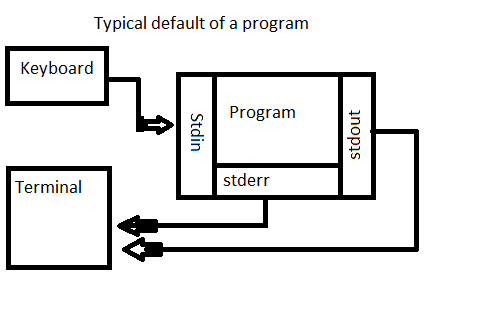
\includegraphics[width=90mm]{stdin_err_out_example.png}
	        \caption{Illustration of default stdin, stdout, and stderr.}
        \end{figure}
     
         
        Redirection and pipes have to do with telling the shell to set stdin, stdout, or stderr to something other then these defaults, such as a file or another program.
    \subsection{Redirection}
        Here is a table of the redirection operators:
        \begin{center}
            \begin{tabular}{|l|l|}
                 \hline
                 program $<$ file1 & stdin is set to file1. \\
                 program $>$ file1 & stdout is set to file1. If file1 does not exist it is created. If it does exist it is overwritten. \\
                 program $>>$ file1 & Same as above but appends instead of overwrites. \\
                 program $2>$ file1 & Same as $>$ but for stderr. \\
                 program $2>>$ file1 & Same as $>>$ but for stderr. \\ \hline
            \end{tabular}
        \end{center}
        \begin{figure}[ht!]
	        \centering
	        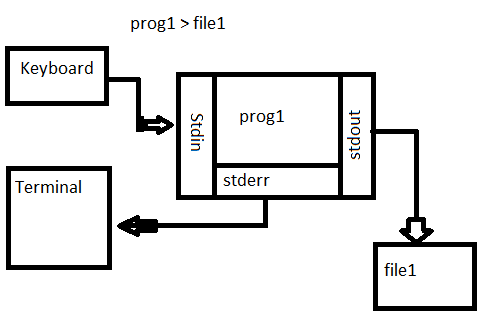
\includegraphics[width=90mm]{redirection_out_example.png}
	        \caption{Illustration of redirecting stdout to file1.} 
        \end{figure}  
        \begin{figure}[ht!]
	        \centering
	        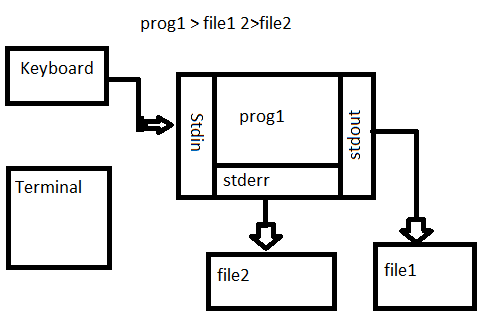
\includegraphics[width=90mm]{redirection_err_example.png}
	        \caption{Illustration of redirecting stdout to file1 and stderr to file2.} 
        \end{figure}
        And the above are to help visualize what happens with redirection.
        
        This might seem like a lot but a few examples will show how easy and helpful this is. Suppose we want to save the list of all the files and directories in our home directory into a file. We can do this with,
        \commandline{ls $\sim$ $>$ myfiles}
        This creates a new file called myfiles, or overwrites it if it already exists, and places it in your current working directory.
        \begin{ex}
            Recall that we discussed how cat can be used with no files as arguments and how it seemed pointless? We can utilize this to quickly make files.
            \begin{enumerate}
                \item Start by running:
                    \commandline{cat $>$ yesFile}
                \item Now type ``y" and then hit ctrl-d.
                \item Now redirect ``yesFile" as input into your greeting.sh program. What happens? What else could you try?
            \end{enumerate}
        \end{ex}
        
        One of the most common ways this shows up is wanting to quickly test your program by making a file for input (like we did in the above exercise) and/or making a file for output. Suppose you have made a python program where you always enter ``yes" then 5 then ``sandwich". You are trying to iron out bugs and are repeatedly running it, finding errors, making changes, and then running it again. We can do this with:
        \commandline{python3 myProgram $<$ testFile}
        Where ``testFile" is our three lines of input. 
        
        Let's look at a few more examples since this is such an important topic. Suppose that we want to delete all \textit{empty directories} in our home directory. One way we can do this is recalling that * is the wildcard character. DON'T FOLLOW ALONG FOR THE COMING COMMANDS. If we run,
        \commandline{rmdir *}
        this will get the job done but you will get an error message for every single file and directory that is not empty. You are now a professional at the command line and know that this will happen and do not want to see possibly hundreds of error messages. Therefore we can do the following,
        \commandline{rmdir * $2>$ /dev/null}
        What we have done is redirected all the error messages into the garbage. ``/dev/null" is a special file, that is actually a file descriptor just like stdin, stdout, and stderr, whose sole purpose is to throw away output like we just did.
 
    \subsection{Pipes}
        Pipes are similar to redirection except that we are changing stdout of one program to now be stdin of another. We can string together as many programs as we would like. Here is the general form:
        \commandline{prog1 $|$ prog2 $|$ prog3 ... $|$ progN}
        Which we can visualize as follows:
        \begin{figure}[ht!]
	        \centering
	        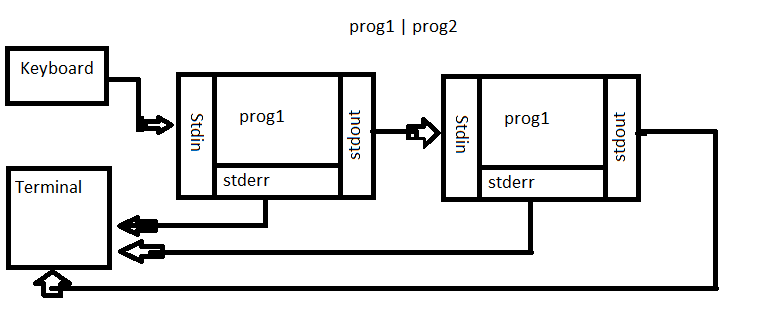
\includegraphics[width=90mm]{pipe_example.png}
	        \caption{An Example Linux Directory Tree.} 
        \end{figure}  
        
        Let's see some examples: Suppose we want to see everything in a directory but it is massive and we want to peruse it we can do so by,
        \commandline{ls bigdir $|$ less}
        this is very helpful on shells with no scrolling features. 
        
        Here is a more advanced example that is interesting and fun but ultimately useless,
        \commandline{find * -name *.c $2>$ /dev/null $|$ xargs cat $|$ grep "if " $|$ wc -l}
        
        \begin{ex}
            With the hint that \textbf{xargs cmd} takes input from stdin and makes them the arguments for cmd, what does the above command do?
        \end{ex}
        
        \begin{ex}
            Suppose we have a file ``largeFile.txt'' which has many lines and each line is quite long. Now suppose that you needed to know how many words were on the first line of that file; what would you run to solve this problem?
        \end{ex}
        
        \begin{ex}
            How could you achieve the same goal as our first example:
            \commandline{ls bigdir $|$ less}
            but without using pipes?
        \end{ex}
        
        \begin{ex}
            We just saw how to rework a pipe into a redirection. A lot of times we can rework a redirection into a pipe. Try to achieve the same goal that ``yesfile" accomplished but without using any files or redirection. Hint: Start by running the following:
                \commandline{man yes}
        \end{ex}
        
        \begin{ex}
            Find the number of computer science students who do not have a unique first 5 characters of last name followed first character of first name username. Hint: if this is the case then the username on the computer will end with a digit. Hint2: This regular expression ``[1-9]" is true if there is at least one digit between '1' and '9'; and [a-z] is true if there is at least 1 character between 'a' and 'z'.
        \end{ex}
        
        \begin{ex}
            Use ``man" and the knowledge gained in the last two workshops to decipher this line. 
            \commandline{cut -d':' /etc/passwd -f7 $|$ sort $|$ uniq -c $|$ sort -b -h -r}
            What is the end result telling us? Why did I do each part? \textbf{Hint}: Try running just the cut command, then the cut piped into sort command, etc $\dots$ seeing how each program changes the output helps to understand what the whole line is doing.\textbf{Note}: \textbf{cut, sort,} and \textbf{uniq} are called filter; this example's intention is to illustrate why.
        \end{ex}
        
        

\section{Processes and Jobs}
    A running program is called a process. Unix and Unix-like operating systems are multitasking and multiuser operating system meaning that at any time many different users can be running many different processes. For example I can be running two Firefox browsers while running a command on the command line and also have music being played. At the same time someone can be using the computer through an ssh connection and they themselves can be running multiple programs.
    
\subsection{Viewing Processes and Users}
    The \textbf{who} program allows you to see all other uses that are currently logged on. Just type:
    \commandline{who}
    and maybe the output is:
    \exampleout{tarquib pts/0 2016-04-10 13:37 (140.160.117.111)}
    \exampleout{birchr  pts/2 2016-04-04 13:21 (tmux(2683).\%0)}
    Showing that there are two users logged in in $tarquib$ and $birchr$ and the former is sshed in from a different ip address while the latter is using the terminal tmux. We can also see when each user logged in. The \textbf{man} page for this program is very digestible if you want to learn more.
    
    To see all processes running in a dynamic updating way with the most intensive processes listed first run \textbf{top} or \textbf{htop}. To leave type ``q". A static but very robust and more universal program is \textbf{ps}. To see all programs you are running enter:
    \commandline{ps -u}
    And you will see something like this:
\begin{code}
    USER       PID %CPU %MEM    VSZ   RSS TTY      STAT START   TIME COMMAND
    tarquib  24130  0.0  0.0  16280  6596 pts/4    Ss   13:37   0:00 -bash
    tarquib  24810  0.0  0.0  10660  2292 pts/4    R+   14:16   0:00 ps -u
\end{code}
    Notice that the process for the command itself is shown in the table. You can also see all the processes of all users including root processes with:
    \commandline{ps -aux}
    There is a lot more to the \textbf{ps} command then we can cover. Try reading through the \textbf{man} page although it might be harder to sift through then some of the others we have looked at. You can also search the Internet for ``ps command" in order to find a slew of guides to the most common option such as this one: \url{http://www.binarytides.com/linux-ps-command/}
    
    
\subsection{Using jobs in Bash}
    Bash has a concept of foreground and background jobs. We have actually already seen how to open a program in the background:
    \commandline{program options \&}
    \exampleout{[num] num2}
    Where num1 is the $jobid$ and the num2 is the $processid$ which is commonly abbreviated as $PID$.
    For example:
    \commandline{firefox \&}
    \exampleout{[1] 6044}
    will open up Firefox and have it run in the background so that you can still enter commands on the command line. 
    
    You can see all running jobs with:
    \commandline{jobs}
    To move a job into the foreground enter:
    \commandline{fg jobid}
    
    \textbf{Note} that a program put in the background may still use stdout, stderr, and stdin. This can cause confusing results where text will apear on the screen when you are in the middle of typing a command. Normally we run commands that either do not use these such as Firefox or we use redirection and pipes to suppress these. 

\subsection{Killing Processes}
    Now that we have the basics or jobs and processes lets see how we can quit processes. Unix using the morbid terminology of ``Killing" a process and the corresponding command is \textbf{kill}. \textbf{kill} actually is used to send any ``SIGNAL" to a program but we will only concern ourselves with the kill signal for now (you will learn more about SIGNALS in \textit{CSCI 352}). 
    
    First find the PID of the process you want to kill using \textbf{ps}, \textbf{jobs}, or one of the ``top" programs we have already discussed. Now enter:
    \commandline{kill -9 PID}
    
    Alternatively you can use \textbf{pkill}, which is short for \textbf{p}rocess \textbf{kill}, to kill a process based off its name. It has the following format:
    \commandline{pkill processname}
    
    \begin{ex}
        Let's explore jobs and discover a limitation of pkill.
        \begin{enumerate}
            \item Open up two processes of the program \textbf{kate}. Note that there is only one program \textbf{kate} but there is multiple processes of the program \textbf{kate}, this is similar to the difference between objects and classes. We can accomplish this with one line as follows:
            \commandline{kate \& kate \&}
            \item See the jobs by using the \textbf{jobs} command.
            \item Now use \textbf{pkill} to kill \textbf{kate}. What happens?
            \item What if we only wanted to kill one of the text editor windows and not both? 
        \end{enumerate}
    \end{ex}

\chapter{More to Learn!}
We have learned a lot about how to use the command line in the last two workshops. If there was a ``Bash 3" workshop it would most likely cover some of the following:
\begin{itemize}
        \item Archives and Compression:
            \begin{itemize}
                \item{\textbf{tar}} A program to make archive files. This allows you to bundle related files into one file that can be saved or sent to someone else. Some of the professors here require work be submitted in a tar file.
                \item{\textbf{gzip}, \textbf{gunzip}, \textbf{zip}, \textbf{gzip2}, \textbf{gunzip2:}} Here is short list of Unix file compression utilities where some are better at compression but slower while others are the opposite. \textbf{zip} is the command utility to make ``zip" files which are the most common compression format on windows. The others are more geared toward Unix systems.
            \end{itemize}
            
        \item Links: What are hard and soft links and how do they differ. How to use the \textbf{link} command. Some of this is covered in \textit{CSCI 352}.
        \item More on regular expressions: The theory will be discussed in \textit{CSCI 301} but the Unix dialect of regular expression may or may not. It is never to early to learn about how to apply this concise and powerful language of describing strings.
        \item{\textit{./bashrc} :} Look for this file in your home directory (remember to use ``ls -a" since it is hidden). This file is used to customize your bash environment. You can change your prompt to be super fancy, use \textbf{alias} to make shortcuts for your favorite commands and arguments, change your \textit{shell variables} such as \$PATH, and much more. Search online for cool ``./bashrc" files or read tutorials on how to make your own that is just right for you!
        \item{System Monitoring:} Look up \textbf{top}, \textbf{htop}, \textbf{who}, and \textbf{free}. These command allow you to see which processes are using the most resources, who is currently logged in, and how much ram is being used. There are a lot of other programs designed for system admins and users who want to know more about what there computer is doing.
\end{itemize}

\newpage

And for the truly committed: 
\begin{itemize}
        \item{Find your text editor:} Master either \textbf{vim} or \textbf{emacs} so you can write code and edit files efficiently without leaving the command line. Mastering an editor designed for program will allow you to finish your assignments quicker and help you for the rest of your career. \textbf{We will be offering workshops in both of these this quarter!}
        \item{C Development:} Here are some common C development programs: \textbf{gdb}, \textbf{make},
            \textbf{configure},\textbf{gcc} or \textbf{clang}. C and Unix were made by the same researchers mostly in conjunction with one another. Thus C development tools are abundant for the command line. \textbf{Look for our workshops in C, gdb, make, and Valgrind this quarter for more on command line development of C programs}.
        \item{Networking}
            \begin{itemize}
                \item{\textbf{ssh}} We briefly discussed this in the first workshop. Learn more about how this can be configured so you don't have to enter your credentials each time or how you can use it to push a pull to your github.com account. \textbf{We will be having a workshop on Git this quarter.}
                \item{\textbf{telnet}} Send information across the Internet or LAN to other Unix computers. This will be used a lot in     \textit{CSCI 367}.
                \item{\textbf{ping}} This program comes in handy to check your Internet connection. Run \commandline{ping -c 3 www.google.com} to see if you can receive a response from Google. If this fails ( ``100\% packet loss") you need to try to fix your Internet connection. May not work on lab machines.
            \end{itemize}

        \item Text processing:
            \begin{itemize}
                \item{\textbf{sed:} } A \textbf{s}tream \textbf{ed}itor which manipulates text from a stream of text.  
                \item{\textbf{awk:}} An interpreted language developed a Bell Labs (the makers of Unix and C!) for writing programs to manipulate text. Many powerful text filters can be made in one line using this programming language and is often used directly from the command line or incorporated intro scripts.
                \item{\textbf{perl:}} This is a full blown interpreted programming language similar to languages like Python. This language is know for having many ways to write the same program including many interesting and powerful one line programs that can be incorporated in shell scripts.  
            \end{itemize}
        \item{So much more!} There are thousands of command line programs on a standard installation of Linux, OSX, or any other Unix or Unix like Operating System (BSD, freeBSD, netBSD, DragonFlyBSD, Soloras, ect \dots). Many of these are for specific purposes such as networking (\textbf{ftp}, \dots), servers (\textbf{apache}, \dots), databases, system administration task, advance software development. Others are for common task such email, calenders, calculators, ect \dots but these are now mostly done with GUI's even by the most dedicated Bash users. 
\end{itemize}

\section{Retrospective and Closing Comments}

We have covered enough in the last two workshops that you should feel comfortable writing programs and doing many task related to the topics you will learn in the Computer Science degree through the command line. If you are curious and eager to learn more about the command line then we encourage you to use the \textbf{man} pages and your favorite search engine to look into the tools and topics that we just outlined. Also note that you will learn a lot from friends, teachers, and colleagues in the common years if you continue in the CSCI program. 

\newpage
\section{\\Glossary} \label{App:AppendixB}
% the \\ insures the section title is centered below the phrase: Appendix B

Glossary of terms will be added later.

\newpage
\begin{thebibliography}{10}

	\bibitem{Figure 1} Figure 1 found at http://www.linuxtrainingacademy.com/wp-content/uploads/2014/03/linux-directory-tree.jpg \\

\end{thebibliography}



\end{document}
